\documentclass[letterpaper,10pt]{article}

% Soporte para los acentos.
\usepackage[utf8]{inputenc}
\usepackage[T1]{fontenc}
% Idioma español.
\usepackage[spanish,mexico, es-tabla]{babel}
% Soporte de símbolos adicionales (matemáticas)
\usepackage{multirow}
\usepackage{amsmath}
\usepackage{amssymb}
\usepackage{amsthm}
\usepackage{amsfonts}
\usepackage{latexsym}
\usepackage{enumerate}
\usepackage{ragged2e}
% Soporte para imágenes.
\usepackage{graphicx}
% Soporte para código.
\usepackage{listings}
% Soporte para URL.
\usepackage{hyperref}
\usepackage[all]{xy} %para diagramas conmutativos
% Modificamos los márgenes del documento.
\usepackage[lmargin=2cm,rmargin=2cm,top=2cm,bottom=2cm]{geometry}
\title{Autómatas y Lenguajes Formales \\ Tarea 8}
\author{González Montiel Luis Fernando\\ García Pérez Isai Uzziel\\}
\date{\today}

\begin{document}
\maketitle

	\begin{enumerate}

	 % Ejercicio 1.
    \item Diseñe una máquina de Turing determinista, especificando cada uno de sus siete elementos a detalle, de manera que reconozca el lenguaje A = $\lbrace$ $a^{2n}$ $\mid$ n $\geq$ 0 $\rbrace$ , el lenguaje que consiste de todas
las cadenas de a’s cuya longitud es una potencia de 2. Una idea para definir la función de transición
es el siguiente proceso iterativo:\\ \\
	I. Acepte la cadena si hay un a en la cinta.\\
	II. Si hay más de un a en la cinta, marque la a más a la izquierda con una X y busque la
	a más a la derecha, márquela con una Y. Repita esta acción hasta marcar todas las
	a’s, quedarán las X’s a la izquierda y las Y’s a la derecha. Hay dos posibles situaciones:\\
	a) Se encuentra actualmente buscando la a más a la izquierda pero todas las a’s ya
	están marcadas. Entonces la cadena de a’s con la que se inició esta iteración es
	de longitud par. Convierta todas las Y’s a $\sqcup$ y las X’s en a. Posicione la cabeza
	lectora en la a más a la izquierda y vuelva al paso I.\\
	b) Se encuentra actualmente buscando la a más a la derecha pero todas las a’s ya
	están marcadas. Entonces la cadena de a’s con la que se inició esta iteración es
	de longitud impar. Debe detenerse rechazando.\\
La noción básica en el proceso anterior es ir dividiendo entre dos la cadena de a’s en la cinta a cada
paso de la iteración.
   
    \textsc{Solución:}
    \\  
	M2 = En la cadena de entrada w:\\
	1.- Deslizamos de izquierda a derecha por la cinta, tachando cada 2 a's.\\
	2.- Si en la etapa 1 la cinta contenía una sola a, se acepta.\\
	3.- Si en la etapa 1 la cinta contenía más de una a y el númmero  de a's era impar, se rechaza.\\
	4.- Regresamos la cabeza al extremo izquierdo de la cinta.\\
	5.- Vamos al paso 1.\\
	Corremos la MT M2 con la entrada aaaa.\\
	Al inicio contiene la entrada aaaa.\\
	$\rightarrow$aaaa$\cdots$\\
	1: Nos movemos de izquierda a derecha por la cinta, tachando cada 2 a's\\
		 $\sqcup$xax$\rightarrow$ $\sqcup$ $\cdots$ (Ponemos $\sqcup$ al inicio de la celda para marcar el inicio de la cinta).\\
	Etapa4: Regresamos la cabeza al extremo izquierdo de la cinta (Marcada por $\sqcup$ )\\
	$\rightarrow$  $\sqcup$xax$\sqcup$ $\cdots$ \\
	Etapa1: Nos movemos de izquierda a derecha sobre la cinta, tachando cada 2 a's. \\
	$\sqcup$xxx$\rightarrow$ $\sqcup$ $\cdots$\\
	Corremos la etapa 4 y 1: Regresamos la cabeza al extremo izquierdo y escaneamos la cinta.\\
	Corremos la etapa2: Si en la etapa 1 la cinta contiene una sola a, aceptamos.
	\\
	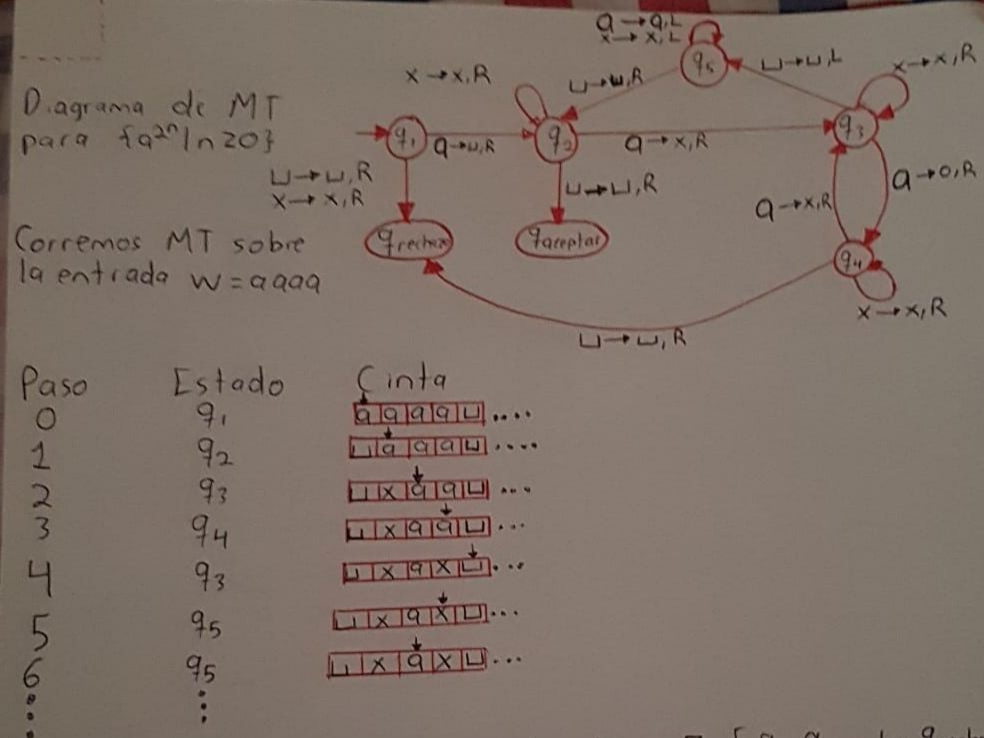
\includegraphics[width=8cm, height=5cm]{imagenuno}
	\\
	MT para $\lbrace$ $a^{2n}$ $\mid$ n $\geq$ 0 $\rbrace$, MT M2= (Q, $\Sigma$, $\Gamma$, $\delta$, q , $q_{acepta}$, $q_{rechaza}$)donde: \\
	$\cdot$) Q = $\lbrace$q1, q2, q3, q4, q5, $q_{acepta}$, $q_{rechaza}$)\\
	$\cdot$) $\Sigma$ = $\lbrace$q$\rbrace$\\
	$\cdot$) $\Gamma$ = $\lbrace$a, x, $\sqcup$ $\rbrace$
	$\cdot$) q1$\rightarrow$estado inicial\\
	$\cdot$) $q_{acepta}$ $\rightarrow$ estado de aceptación\\
	$\cdot$)  $q_{rechaza}$ $\rightarrow$ estado de rechazo\\
	$\cdot$) $\delta$ : Q $\times$ $\Gamma$ $\rightarrow$ Q $\times$ $\Gamma$ $\times$ $\lbrace$L, R$\rbrace$, por ejemplo:\\
	$\delta$(q4,a) = (q3,x,R)\\
	$\delta$(q3,$\sqcup$) = (q5,$\sqcup$,L)
	
	
    % Ejercicio 2.
    \item Para los propósitos de este problema, si está describiendo una Máquina de Turing, no
es necesario que especifique los elementos de la tupla. Una descripción correcta, precisa y clara es
suficiente. Muestre que los lenguajes recursivamente enumerables son cerrados bajo la operación de
reversa.

    \textsc{Solución:}
    \\
    Sea L un lenguaje recursivamente enumerable, tiene una MT M que reconoce a L. Contruimos una MT $M^{R}$ tal que q0' $\in$ $M^{R}$ $\neq$ q0 $\in$ M y además $\delta$(q0, i, R)$\forall$i estando en los símbolos de M menos el vacío. Es decir, avanzamos a la derecha con cualquier símbolo menos con el vacío.
    Definimos la transición para que cuando llegue al vacío vaya a la izquierda y cambiamos el estado original inicial.\\
    $\delta$(q0,$\sqcup$) = $\delta$($q_{inicial}$, $\sqcup$, L) con $q_{inicial}$ $\in$ $M^{R}$, así la cabeza lectora empieza en el final en lugar del inicio.\\
    Por cada transición, creamos unas nuevas en las que cambiamos R por la L y L por R.\\
    Ahora nos tomamos una cadena w$\in$L, veamos que MT $M^{R}$ acepta $w^{R}$. Suponemos que existe una ruta de aceptación en los estados en los símbolos. Veremos que a partir de que sede el control al estado original, la ruta de aceptación es igual en ambos casos. Por ejemplo la MT que acepta a*b*, ab, su ruta de ejecución sería q0,a $\rightarrow$q0,b$\rightarrow$q0,$\sqcup$ $\rightarrow$ $qf_{acepta}$.\\
    Lo que se propone es que a partir de cierto punto las rutas de ejecución de ambas máquinas serán iguales, razón por la que funciona. Además, como sabemos que en un punto las rutas de ejecución siempre serán iguales, terminarán en lo mismo, es decir, ambas terminan ya sea en un estado de aceptación o uno de rechazo.\\
    $\therefore$ w$\in$L, MT $M^{R}$ acepta $w^{R}$.
    
	
    % Ejercicio 3.
    \item Suponga que T es una máquina de Turing que acepta el lenguaje L. Describa cómo construir
una máquina de Turing no determinista que acepte L*.
    
    \textsc{Solución:}
    \\
    Insertamos un espacio en blanco no determinista en cualquier posición de la cadena de entrada, incluso al principio y al final.
    Con la cabeza de la cinta en el espacio en blanco y se ejecuta, aceptamos la entrada nula; de lo contrario, comience en el extremo derecho de la entrada y repita la siguiente operación, un número (quizá cero) de veces e inserte un spacio en blano en alguna posición y ejecute. T en la parte de la cadena a la derecha del espacio en blanco; si T acepta borramos todo lo que la última iteración de ésta operación, movemos la cabeza de la cina al principio de la cinta y ejecutamos T una vez más en la entrada restante.
    \\
	
	 % Ejercicio 4.
    \item Una máquina de Turing con movimiento neutro es una MT determinista convencional
donde los movimientos permitidos son izquierda (L), derecha (D) y neutro (N). Realizar un movimiento neutro quiere decir que la cabeza lectora permanece inmóvil al realizar una transición. 
Así su función de transición es $\delta$ : Q $\times$ $\Gamma$ $\rightarrow$ Q $\times$ $\Gamma$ $\times$ $\lbrace$L, N, D$\rbrace$. 
Demuestre que esta variante de la máquina de Turing es equivalente a su definición convencional. ¿Cómo es que se puede simular un movimiento neutro a través de movimientos L y R?
    
    \textsc{Solución:}
    \\
    Dada una MT convensional simularemos una MT con movimiento neutro.
    Usando la función de transición, tendríamos $\delta$(q,X) = (p,X,R) y luego regresaría con...\\
    $\delta$(p,X) = (p,X,L) así se quedaría igual porque la cabeza lectora se mueve y se regresa y eso mismo hace que quede intacto el contenido de la cinta.\\
    Y por otra parte, sí sería posible simular una MT con movimiento neutro con una convencional pues por definición una MT con movimiento neutro engloba todo lo que hace una MT convencional.\\
        
    % Ejercicio 5.
    \item Demuestre que el lenguaje $\overline{L_{d} }$ es recursivamente enumerable pero no es recursivo.
    
    \textsc{Solución:}
    \\
    Sin pérdida de generalidad asumiendo que $\overline{L_{d} }$ no es recusrivamente enumerable, lo demostramos por contradicción.\\
    ATM = $\lbrace$ $\langle$M,w$\rangle$ $\vert$ M es una MT y M acepta a w$\rbrace$.\\
    ATM es r.e. pero no es recursivo, entonce hay una MT que siempre detiene y L(M) = ATM.\\
    On input i\\
    Run M on input $\langle$i,i$\rangle$\\
    output "si" si i rechaza i\\
    output "no" si i acepta i\\
    Observemos que L(D) = $L_{d}$.\\Pero $L_{d}$ no es r.e. lo que nos resulta una contradicción.\\
    $\therefore$ Es no recursivo como también vimos.\\
    
   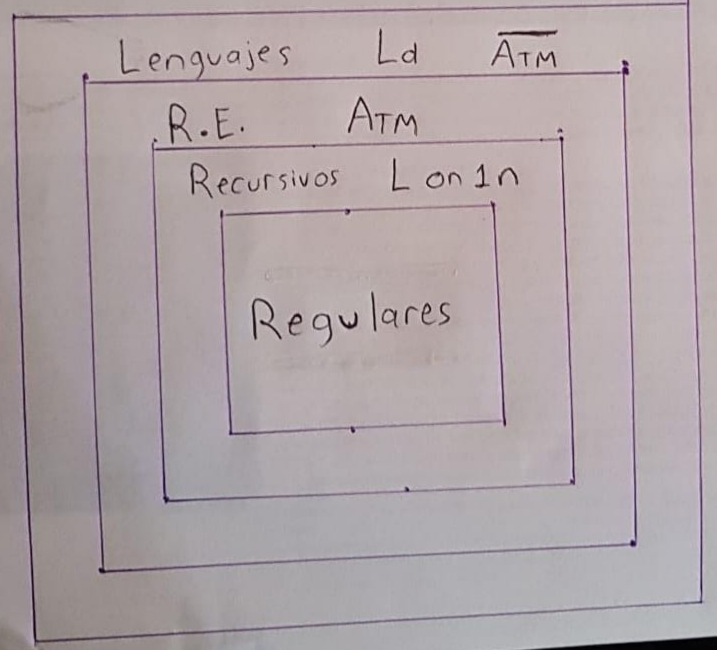
\includegraphics[width=8cm, height=5cm]{imagen}
    
    % Ejercicio 6.
    \item Por medio de una reducción demuestre que el lenguaje $L^{ \lozenge }$ = $\lbrace$N $\mid$ N es una MT y L(N) es un lenguaje recursivo $\rbrace$ no es recursivo.
    
    \textsc{Solución:}
    \\
    

	\end{enumerate} 
\end{document}
